% Document : compte rendu des DM
% Auteur : Xavier Gandibleux
% Année académique : 2018-2019

\documentclass[a4paper,10pt]{article}
\usepackage{tikz}


% passe en mode large sur la page A4
\usepackage{a4wide} 

% document francisé
\usepackage[polutonikogreek,english,francais]{babel} 

% permet la frappe de caracteres accentues (sur macOS)
%\usepackage[utf8x]{inputenc} 

\usepackage{graphicx,float,subcaption} % figure et placement de figure
\usepackage[top=10mm, bottom=10mm, left=20mm, right=20mm]{geometry}

\usepackage[linesnumbered,frenchkw,ruled,french]{algorithm2e}

\usepackage{verbatim}
\usepackage{fancyvrb}
\usepackage[T1]{fontenc}
%\usepackage{graphicx}
%\usepackage{grffile}
%\usepackage{longtable}
%\usepackage{wrapfig}
%\usepackage{rotating}
%\usepackage[normalem]{ulem}
%\usepackage{amsmath}
%\usepackage{textcomp}
%\usepackage{amssymb}
%\usepackage{capt-of}
\usepackage{hyperref}% \documentclass[a4paper,11pt]{article}
%\usepackage[margin=2cm]{geometry}
\usepackage[utf8]{inputenc}

\usepackage{color}
\usepackage{xcolor}

\usepackage[]{amsmath,amsfonts,amssymb,stmaryrd,amsthm}
%\usepackage{fullpage}
%\usepackage{multirow}
%\usepackage[rounded]{syntax}
%\usepackage[section]{placeins}
\newtheorem{example}{Exemple} %%% modifier ici si on veut en fr/en

\usepackage{todonotes}
\usepackage{listings} 


\usepackage{listings}
\usepackage{inconsolata} % very nice fixed-width font included with texlive-full
%\usepackage[usenames,dvipsnames]{color} % more flexible names for syntax highlighting colors

\definecolor{chameleond}{HTML}{4E9A06}
\definecolor{skyblued}{HTML}{204A87}
\definecolor{darkgreen}{HTML}{006400}

%\usepackage[usenames,dvipsnames]{color} % more flexible names for syntax highlighting colors


\lstset{
basicstyle=\ttfamily, 
columns=fullflexible, % make sure to use fixed-width font, CM typewriter is NOT fixed width
numbers=left, 
numberstyle=\small\ttfamily\color{gray},
stepnumber=1,              
numbersep=10pt, 
numberfirstline=true, 
numberblanklines=true, 
tabsize=4,
lineskip=-1.5pt,
extendedchars=true,
breaklines=true,        
keywordstyle=\color{skyblued}\bfseries,
identifierstyle=, % using emph or index keywords
commentstyle=\sffamily\color{darkgreen},
stringstyle=\color{chameleond},
showstringspaces=false,
showtabs=false,
upquote=false,
texcl=true % interpet comments as LaTeX
}


\lstset{literate=
  {α}{{$\alpha$}}1 {Δ}{{$\Delta$}}1
  {á}{{\'a}}1 {é}{{\'e}}1 {í}{{\'i}}1 {ó}{{\'o}}1 {ú}{{\'u}}1
  {Á}{{\'A}}1 {É}{{\'E}}1 {Í}{{\'I}}1 {Ó}{{\'O}}1 {Ú}{{\'U}}1
  {à}{{\`a}}1 {è}{{\`e}}1 {ì}{{\`i}}1 {ò}{{\`o}}1 {ù}{{\`u}}1
  {À}{{\`A}}1 {È}{{\'E}}1 {Ì}{{\`I}}1 {Ò}{{\`O}}1 {Ù}{{\`U}}1
  {ä}{{\"a}}1 {ë}{{\"e}}1 {ï}{{\"i}}1 {ö}{{\"o}}1 {ü}{{\"u}}1
  {Ä}{{\"A}}1 {Ë}{{\"E}}1 {Ï}{{\"I}}1 {Ö}{{\"O}}1 {Ü}{{\"U}}1
  {â}{{\^a}}1 {ê}{{\^e}}1 {î}{{\^i}}1 {ô}{{\^o}}1 {û}{{\^u}}1
  {Â}{{\^A}}1 {Ê}{{\^E}}1 {Î}{{\^I}}1 {Ô}{{\^O}}1 {Û}{{\^U}}1
  {œ}{{\oe}}1 {Œ}{{\OE}}1 {æ}{{\ae}}1 {Æ}{{\AE}}1 {ß}{{\ss}}1
  {ű}{{\H{u}}}1 {Ű}{{\H{U}}}1 {ő}{{\H{o}}}1 {Ő}{{\H{O}}}1
  {ç}{{\c c}}1 {Ç}{{\c C}}1 {ø}{{\o}}1 {å}{{\r a}}1 {Å}{{\r A}}1
  {€}{{\EUR}}1 {£}{{\pounds}}1
}

% \lstset{language=bash,
% stringstyle=\ttfamily,
% basicstyle=\footnotesize, 
% showstringspaces=false,
% breaklines=true,
% }

\lstdefinestyle{numbers} {numbers=left, stepnumber=5, numberstyle=\tiny, numbersep=10pt}
% \lstdefinestyle{lc3} {language=[x86masm]Assembler,style=numbers,frame=lines,showstringspaces=false,keywords={BR,LD,BRz,BRn,BRzp,BRnz,BRnzp,LEA,HALT,RET,.END,.ORIG,.FILL,.STRINGZ,PUTS,ADD,AND,OR,OUT,NOT,LDR,STR,JSR,NOP,GETC},showstringspaces=false,keepspaces=true,flexiblecolumns=true,deletekeywords={end}}

\lstdefinestyle{target}
{language=[x86masm]Assembler,style=numbers,frame=lines,showstringspaces=false,keywords={add,
  jump, snif,call,return,.string,.reserve,.word,.set,.align16,letl,leth,.let,and,or,wmem,rmem,asr,xor,sub,sgt,sle,slt,slt},showstringspaces=false,keepspaces=true,flexiblecolumns=true,deletekeywords={end},breaklines=true}



%\definecolor{chameleond}{HTML}{4E9A06}
%\definecolor{skyblued}{HTML}{204A87}


\lstdefinestyle{digmips} {language=[x86masm]Assembler,style=numbers,frame=lines,showstringspaces=false,keywords={add,sub,ld,ldi,ble,j,jmp,st},showstringspaces=false,keepspaces=true,flexiblecolumns=true,deletekeywords={end},keywordstyle=\color{skyblued},commentstyle=\color{red}\bf,morecomment=[l][\color{red}]{//}}


\lstdefinestyle{lc3} {language=[x86masm]Assembler,style=numbers,frame=lines,showstringspaces=false,keywords={BR,LD,BRz,BRn,BRzp,BRnz,BRnzp,LEA,HALT,RET,.END,.ORIG,.FILL,.STRINGZ,PUTS,ADD,AND,OR,OUT,NOT,LDR,STR,JSR,NOP,GETC},showstringspaces=false,keepspaces=true,flexiblecolumns=true,deletekeywords={end}}


\lstdefinelanguage{[Objective]Caml}
{basicstyle=\ttfamily,
keywordstyle=\itshape\bfseries,
identifierstyle=,
stringstyle=\itshape,
commentstyle=\itshape,
flexiblecolumns=true,
escapechar=\%}

\lstdefinelanguage{julia}
{
  keywordsprefix=\@,
  morekeywords={
    exit,whos,edit,load,is,isa,isequal,typeof,tuple,ntuple,uid,hash,finalizer,convert,promote,
    subtype,typemin,typemax,realmin,realmax,sizeof,eps,promote_type,method_exists,applicable,
    invoke,dlopen,dlsym,system,error,throw,assert,new,Inf,Nan,pi,im,begin,while,for,in,return,
    break,continue,macro,quote,let,if,elseif,else,try,catch,end,bitstype,ccall,do,using,module,
    import,export,importall,baremodule,immutable,local,global,const,Bool,Int,Int8,Int16,Int32,
    Int64,Uint,Uint8,Uint16,Uint32,Uint64,Float32,Float64,Complex64,Complex128,Any,Nothing,None,
    function,type,typealias,abstract
  },
  sensitive=true,
  morecomment=[l]{\#},
%  morecomment=[s]{# =}{=#},
  morestring=[b]',
  morestring=[b]" 
}

\lstdefinelanguage{cplus}
{
        frame=lines,
	language=C++,
	basicstyle=\tt,
        morecomment=[l][\color{magenta}]{\#},
	keywordstyle=\color{chameleond},
	identifierstyle=\color{black},
        stringstyle=\color{skyblued},
        commentstyle=\color{red},
	tabsize=4,
}


\lstdefinelanguage{mypython}
{
%        frame=lines,
	language=Python,
	basicstyle=\tt,
        morecomment=[l][\color{magenta}]{\#},
	keywordstyle=\color{chameleond},
	identifierstyle=\color{black},
        stringstyle=\color{skyblued},
        commentstyle=\color{red},
	tabsize=4,
        breaklines=true,
}


\lstdefinelanguage{flexbison}
{
        frame=lines,
	language=C,
	basicstyle=\tt,
        keywords={yylex,yyparse,yyline,yytext,yyin},
        morecomment=[l][\color{magenta}]{\#,},
	keywordstyle=\color{chameleond},
	identifierstyle=\color{black},
        stringstyle=\color{skyblued},
        commentstyle=\color{red},
	tabsize=4,
}


\lstdefinelanguage{antlr}
{
%  frame=lines,
  language=Java,
  basicstyle=\tt\scriptsize,
  breaklines=true,%                                      allow line breaks
  moredelim=[s][\color{blue!50!black}\ttfamily]{'}{'},% single quotes in green
  moredelim=*[s][\color{black}\ttfamily]{options}{\}},%  options in black (until trailing })
  commentstyle={\color{gray}\itshape},%                  gray italics for comments
  morecomment=[l]{//},%                                  define // comment
  emph={%
    STRING%                                            literal strings listed here
  },emphstyle={\color{blue}\ttfamily},%              and formatted in
                                %              blue
  keywords={grammar,header,members,skip},
  alsoletter={:,|,;},%
  morekeywords={:,|,;},%                                 define the special characters
  keywordstyle={\color{chameleond}},%                         and format them in black
}


\lstdefinelanguage{mycaml}
{       language=Caml,
        upquote=true,
        columns=flexible,
        keepspaces=true,
        breakindent=0pt,
        basicstyle=\ttfamily,
        breaklines=true,
        keywordstyle=\color{red},
        commentstyle=\color{darkgreen},
        tabsize=2,
        escapechar=\%,
        escapebegin=\color{blue}
        }

\lstdefinelanguage{myhaskell}
{       language=Haskell,
        upquote=true,
        columns=flexible,
        keepspaces=true,
        breakindent=0pt,
        basicstyle=\ttfamily\scriptsize,
        breaklines=true,
        keywordstyle=\color{red},
        commentstyle=\color{darkgreen},
        tabsize=2,
        escapeinside={!}{!},
        escapebegin=!\endgraf\color{gray},
        }



\newcommand\ocamli[1]{\lstinline[language=mycaml,basicstyle=\ttfamily\normalsize]{#1}}
\newcommand\llvminline[1]{\lstinline[language=LLVM,basicstyle=\ttfamily\normalsize]{#1}}
\newcommand\llvmfile[1]{\lstinputlisting[language=LLVM]{#1}}

\lstnewenvironment{llvmc}{
  \lstset{language=llvm,mathescape,
    basicstyle=\ttfamily\small,
    aboveskip={0\baselineskip},
    belowskip=0\baselineskip
  }}{}


\lstdefinelanguage{lustre}
{
  basewidth={0.5em,0.5em},
  % list of keywords
  morekeywords={
    pre,
    fby,
    ->,
    current,
    when,
    node, 
    returns,
    let,
    tel,
    var,
    if,
    then,
    int,
    bool,
  },
  sensitive=false, % keywords are not case-sensitive
  escapeinside={!}{!},          % if you want to add LaTeX within your code
  morecomment=[l]{//}, % l is for line comment
  morecomment=[s]{/*}{*/}, % s is for start and end delimiter
  morestring=[b]", % defines that strings are enclosed in double quotes
  basicstyle=\ttfamily,
  keywordstyle=\bfseries\color{blue!80!black},
  keywordstyle=[2]\bfseries\color{red!50!white},
  commentstyle=\itshape\color{purple!40!black},
  %identifierstyle=\color{blue!80!black},
  stringstyle=\color{orange}
}


\newcommand{\arthur}[1]{\textcolor{violet}{#1}}
\newcommand{\marie}[1]{\textcolor{red}{#1}}
\newcommand{\prof}[1]{\textcolor{gray}{#1}}

% individualisation des parametres de la page
\parskip8pt
\setlength{\topmargin}{-25mm}
\setlength{\textheight}{250mm}

%
% -----------------------------------------------------------------------------------------------------------------------------------------------------
%

\begin{document}

\lstset{language=julia}

\tikzstyle{fleche}=[->,thick,>=latex]
\tikzstyle{noeud}=[circle,fill=violet!20]
\tikzstyle{legende}=[scale = 0.7,pos=0.59]


~
\vspace{50mm}
{\large
\begin{center}
  Université de Nantes --- UFR Sciences et Techniques\\
  Master informatique parcours ``optimisation en recherche opérationnelle (ORO)''\\
  Année académique 2018-2019
  \vspace{30mm}
 
  { \LARGE
 
     Rapport du projet d'Optimisation discrète et combinatoire\\
     \vspace{5mm}
 
     {\huge \textbf{Projet TAN/SNCF}}
     \vspace{5mm}
 
     Marie \textsc{Humbert--Ropers}$^1$ --  Arthur \textsc{Gontier}$^2$
     \vspace{50mm}
  
     \today
  }  
\end{center}
}

\vfill
\break

\tableofcontents

\vfill
\break

\section{Proposition d'évolution de l'infrastructure}
La proposition d'évolution faite concerne une ancienne ligne ferroviaire reliant la Gare de Nantes à Carquefou. Actuellement peu utilisée, cette ligne permettrait de proposer aux habitants de Carquefou et des alentours de se rentre facilement sur Nantes. En effet, d'après une étude \cite{rapport}[page A.76-A.80], les habitants de Carquefou se rendent au travail sur Nantes en voiture. Il est donc envisageable de leur proposer un service de transport en commun les reliant aux grands axes nantais.
Cette ancienne ligne peut aussi être raccordée avec une ligne plus au sud de Nantes qui s'allonge jusqu'à l'aéroport de Nantes. Comme il existe déjà des infrastructures pour le fret et que de nouvelles infrastructures, comme le CHU, sont en construction, nous proposons de faire une ligne qui s'étend de Carquefou jusqu'à l'aéroport nantais, en passant par la Gare de Nantes et le nouveau CHU. La seule partie du réseau à construire serait celle du côté du CHU, puis les nouvelles stations à rajouter. \\
Cette ligne accueillerait un tram-cargo. Le principe est donc que le tram-train puisse être soit mi-voyageur, mi-fret soit complètement voyageur. Entre Carquefou et Nantes, il existe des zones commerciales/industrielles qui peuvent nécessiter d'être desservies. De plus, le lien jusqu'à l'aéroport, qui fait du transport de personnes et de colis, ouvrirait de nouvelles voies plus rapides pour desservir ces colis. Ce point est aussi valide pour la zone de dépot de fret à côté du nouveau CHU. Aussi, nous proposons la possibilité avec plusieurs terminus (Aéroport, Gare de Nantes, CHU et Carquefou), de réaliser plusieurs lignes selon le taux de fréquentation. 


\section{Choix des arrêts}
Pour la modélisation, nous avons réparti les habitations en petites zones, qui sont au moins partiellement à moins de 500 mètres de la ligne. Dans un second temps, nous avons estimé les populations de ces zones en comptant pour une maison 4 habitants puis pour un appartement 2 habitants. Cela nous a mené à créer une cinquantaine de zones autour de la ligne, certaines habitées, d'autres non. Nous avons ainsi pu fournir des données pour notre problème. Une vue d'ensemble est donnée par la Figure 1.

\begin{figure}[!h]
  \centering
  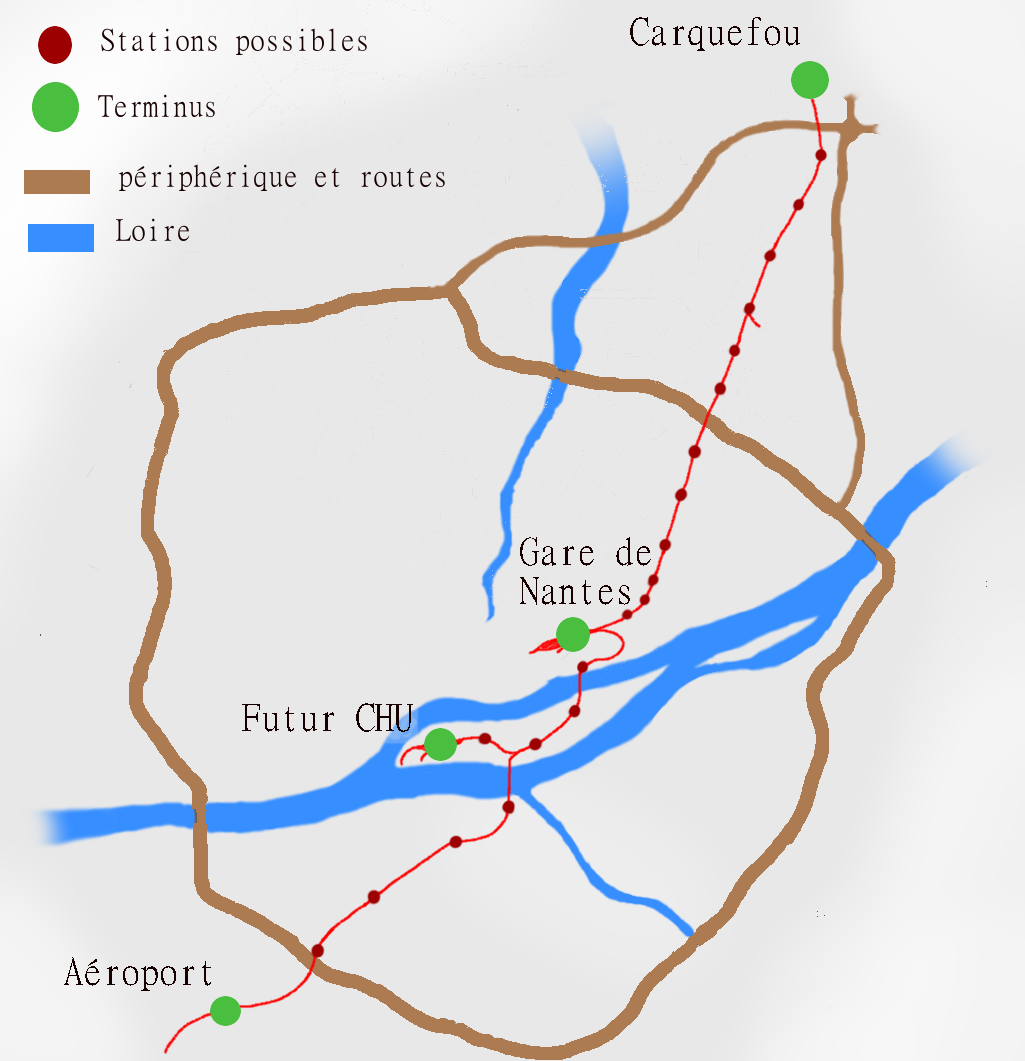
\includegraphics[scale = 0.3]{tramcargo4.png}
  \caption{Schéma de la ligne de tram-cargo envisagée}
\end{figure}

\newpage
Le problème à résoudre est le suivant : On demande à ouvrir un certain nombre p de stations s. Chaque station s dessert certaines zones x de foyers de population, l'ensemble C[s] les rassemble. L'objectif est de maximiser le nombre d'habitants qui auront accès à la ligne tout en ouvrant au maximum p stations.  
 
Le modèle est le suivant :
$$ max \sum s_i h_i$$
$$s.t \sum_{j\in C[i]} x_j -s_i \geq 0,\quad  \forall i \in \{1,...,nb\}$$
$$ \sum_{j\in \{1,...,jmax\} } x_j \leq p $$
$$ x_j \geq 0, \quad \forall j \in \{1,...,jmax\}$$
$$ s_i \geq 0, \quad \forall i \in \{1,...,nb\}$$


Sur cette figure, on mentionne les différentes stations possibles, retenues selon l'un des trois critères : soit il y a une zone dense de population proche, soit il existe dèjà un arrêt, soit la zone est commerciale. On note que dans le modèle actuel, les stations se font choisir selon le nombre d'habitants dans les zones "recouvertes" par la stations (dans un rayon de 500 m). Ainsi, les zones commerciales ne se font pas forcément desservir. Il est donc nécessaire de contraindre leur variable associée, s'il semble vitale de les intégrer. Nous avons numéroté les stations en partant de Carquefou (1) jusqu'au CHU (19), puis en suivant sur le reste de la ligne pour arriver jusqu'à l'aéroport (24).


Ce problème d'ouverture des stations se résout sous JuMP, avec le solveur GLPK. Nous obtenons l'ouverture des stations suivantes : 1, 4, 9, 11, 14, 16, 17, 19, 20 et 22 avec 87.83\% des habitations desservies. La ligne passe bien par des stations déjà très fréquentées, comme la Gare de Nantes(14). Dans cette disposition, l'aéroport est une station sélectionnée non pas à cause d'une forte densité de population à moins de 500 m. mais parce qu'il a été décidé que cette station était nécessaire. Ainsi, elle a été contrainte à 1, comme pour la station du nouveau CHU.


\section{Modèle du LPP}
Sur cette partie, nous considérons la nouvelle ligne tram-train Carquefou vers Nantes ainsi que la matrice Origine-Destination associée. Cette matrice contient le flot de passagers montant/descendant d'une station. (Pour la suite, les données utilisées sont celles pourvues en cours par M.Gandibleux). À partir de ces données, nous réalisons un prétraitement afin de décrire ensuite le modèle du LPP.

\subsection{Prétraitement}

À partir de la matrice OD et du graphe des stations, on établit le voisinage $N(e)$, c'est-à-dire toutes les lignes passant par une même arête. On estime que la fréquence minimum $F_e$ par arête est 5. Pour obtenir la capacité $C_e$ de chaque arête à desservir, il est nécessaire d'explorer le graphe de la manière suivante :
Dans le cas général, la capacité $C_e$ qui doit pouvoir être transportée sur une arête est calculée avec la somme de tous les passagers dont le chemin passe par la dite arête. Considérant que les passagers prennent le plus court chemin, on a besoin d'un algorithme pour calculer celui-ci (par exemple Dijkstra). Mais dans notre cas, le Graphe est un arbre, donc il est possible de simplement le couper en deux sur l'arête e dont on cherche le $C_e$ et calculer la somme de tous les passagers qui partent d'un coté pour aller vers l'autre (et donc empruntent l'arête)
Dans un second temps, une matrice de 0 et de 1 permet de définir la présence des différents couples (l $\times$ f $\times$ c), c'est-à-dire que chaque colonne de la matrice correspond à un couple et au niveau des lignes de la matrice, il y a toutes les possibilités de f puis toutes celles de c puis celles de l représentées. Ainsi, dans chaque colonne, toutes les valeurs sont à 0 sauf à l'intersection des colonnes de f,c,l égal chacune à l'une des valeurs du couple (l $\times$ f $\times$ c)     

\subsection{Description du modèle}
Dans un contexte où il est possible d'envisager plusieurs lignes l différentes, nous supposons pour chaque ligne l plusieurs fréquences f possibles et différents nombres de rames c possibles. À chaque triplet $(l \times f \times c)$ est associé une variable binaire, l'objectif est de déterminer quelle(s) ligne(s) ouvrir avec quelle(s) fréquence(s) et quel nombre de rames.

Le modèle est le suivant, issus de Goossens\cite{goossens2004branch} :
$$ min \sum k_i x_i$$
$$s.t \sum_{i\in N(e)} f_i x_i \geq F_e,  \quad \forall e$$
$$ \sum_{i\in N(e)} f_i c_i x_i \geq C_e, \quad \forall e$$
$$ \sum_{l_j} x_i \leq 1 \forall l_j$$
$$ x_i \geq 0, \quad \forall i \in \{0,1\}$$

Avec : 
\begin{itemize}
  \item $N(e)$ l'ensemble des triplets $(l,f,c)=i$ dont la ligne l passe par l'arrête e.
  \item $F_e$ la fréquence minimale sur une arête e (par défaut 5 toutes les 2 heures)
  \item $C_e$ la capacité à desservir sur l'arête e (cf prétraitement)
  \item $f_i$ la fréquence des trains passant sur la ligne $l_i$
  \item $c_i$ la capacité des trains passant sur la ligne $l_i$
  \item $x_i$ variable binaire représentent l'utilisation ou pas d'un triplet $(l,f,c)=i$, l'unicité des lignes est assurée par le troisième lot de contraintes de type SPP
  \item $k_i$ coût d'utilisation du triplet $(l,f,c)=i$ avec $k_i =$ coût fixe des trains $\times$ temps de parcours $\times$ nombre de rames déployées $+$ coût distance des trains $\times $ distance $\times$ fréquence
\end{itemize}


\paragraph{Remarques:}
\begin{itemize}
\item Nous avons remarqué que modifier légèrement la fonction objectif peut complètement changer les solutions optimales. En effet, en fonction de la valeur de l'économie faite avec l'utilisation des doubles rames, elles seront systématiquement choisies même si la capacité de transport devient surdimentionnée ou jamais choisies. Si on veut une solution qui mélange les deux, on doit régler précisément tous les paramètres ou on doit lancer la résolution sur un réseau avec plus de demandes. On en déduit que la pertinence de cette fonction doit être très précise et cohérente avec la réalité pour obtenir des solutions satisfaisantes au problème.
\item On observe que se sont souvent les contraintes de fréquence qui sont saturées.
\end{itemize}


\newpage
\section{Branch and Bound}
Deux approches du branch \& bound ont été développées : une exploration récusive des noeuds (les noeuds d'une hauteur h sont explorées avant les noeuds de hauteur h + 1) puis une exploration plus intelligente des noeuds.

\subsection{B\&B récursif}
Une fonction récursive permet d'énumérer toutes les branches possibles et pour ne pas tous les explorer, on compare chaque relaxation linéaire à la meilleure borne primale trouvée (que l'on stocke dans une variable globale). On a un algorithme de la forme de l' Algorithme 1 :


\begin{algorithm}[!h]
  \begin{small}
    global primale = infini\;
    \Entree{$contr$,Vecteur des contraintes| $n$,hauteur courante de la récursion}
    \SetKwIF{Si}{SinonSi}{Sinon}{Si}{alors}{Sinon si}{alors}{fin si}{}
    \BlankLine\DontPrintSemicolon
    Résolution de la version LP du problème\;
    \Si{la solution est meilleure que la borne primale}{
      \Si{la solution est entière}{
	mise à jour de la borne primale\;
      }\SinonSi{la solution est réelle}{
	Ajout de la contrainte sur la première variable réelle trouvée\;
        appel récursif contr = 1\;
        appel récursif contr = 0\;
      }
    }
  \end{small}
  \caption{\textbf{Branch \& Bound : Récursif simple}}
\end{algorithm}


\subsection{B\&B choix heuristiques pour les noeuds et variables}
Le Pseudo-code du branch \& bound est le suivant, avec z le coût minimal associée à la solution d'un modèle :

\begin{algorithm}[!h]
  \begin{small}
    \SetKwIF{Si}{SinonSi}{Sinon}{Si}{alors}{Sinon si}{alors}{fin si}{}
    \BlankLine\DontPrintSemicolon
    Borne primale égale à l'infini\;
    Résolution de la version LP du problème\;
    Sauvegarde en mémoire des bornes et des noeuds non sondés\;
    \While{ il y a des noeuds non sondés}{
      Choix du noeud avec le meilleur z (pour un problème min -> un z plus petit)\;
      Choix d'une variable pour faire une nouvelle contrainte \;
      \Pour{ les deux enfants}{
        Résolution de la version LP du problème\;
	\Si{la solution n'est pas entière}{
	  \Si{le z trouvé est moins bon que la borne primale}{
	    Noeud sondé par dominance\;
          }\SinonSi{le z est meilleur}{
	    Noeud pas sondé\;
	  }
        }\SinonSi{la solution est entière}{
	  Noeud sondé\;
	  Mise à jour de la borne primale\;
	}
      }
    }
    \Retour{Borne primale}
  \end{small}
  \caption{\textbf{Branch \& Bound : Avec choix heuristiques}}
\end{algorithm}


Le branch \& bound a été réalisé en se basant sur deux structures de données : un dictionnaire Dico ainsi qu'un Arbre Abr. L'Arbre n'est pas une structure de base de Julia mais une structure créée comme une mutable struct de Julia. Chaque noeud de cet arbre contient un entier et un dictionnaire ayant comme clé un caractère. \\

L'idée derrière l'utilisation de ces deux structures est la suivante : JuMP ne permet pas de supprimer des contraintes ou de changer le signe d'une contrainte ajoutée précédemment, il est donc nécessaire de recréer fréquemment le modèle, en particulier s'il l'on change de branche sans descendre sur un noeud fils (sinon on bénéficie du hot start de JuMP/GLPK). Pour facilement recréer ce modèle, on stocke dans chaque noeud non sondé de l'arbre l'indice de la variable qui sera mise à l'entier supérieur ou inférieur. Dans le dictionnaire de ce même noeud, on créé au plus deux fils : celui se repérant avec 'a' correspond au modèle où la variable prend la valeur de l'entier inférieur. Celui se repérant avec 'b' correspond au modèle où la variable prend la valeur de l'entier supérieur. Les modèles avec les nouvelles contraintes sont calculés et, ceux qui ne sont pas sondés sont rajoutés à l'arbre. La racine se repère par la lettre 'g'. Ainsi, lors du parcours de l'arbre, un modèle avec ses contraintes correspond à un unique mot de la forme suivante : g(a|b)* . \\

Pour ne pas avoir à parcourir tout l'arbre pour retrouver le noeud le plus intéressant à développer, toutes les valeurs des z des noeuds non sondés sont stockées dans le dictionnaire Dico, avec comme clé le parcours dans l'arbre, c'est-à-dire le mot créé précédemment.
Le dictionnaire a pour objectif de stocker les valeurs des coûts minimum des différents noeuds non sondé. Ce dictionnaire est souvent mis à jour pour éviter de prendre un noeud qui pourrait être sondé par dominance. On note que la version implémentée est faite pour les variables binaires mais, qu'en rajoutant une entrée dans l'arbre (prendre de la solution la valeur, noté val, de la variable que l'on veut fixer à un entier), il est possible de facilement modifier les lignes de codes d'concernant l'ajout des contraintes en remplacant <= 0 et >= 1 par, respectivement floor(val) et ceil(val). \\

Dans le cadre de ce branch \& bound, nous avons développé deux méthodes de choix pour les noeuds et les variables. 
Pour les choix de variables, une variable non binaire est recherchée dans la solution du modèle présent dans un noeud (non entière de manière plus large). Nous avons pris en compte pour cela deux possibilités :
\begin{itemize}
\item Pour ne pas parcourir systématiquement toutes les variables d'une solution, prendre la première variable qui n'est pas binaire 
\item Dans l'espoir de réaliser moins de noeuds, faire le choix de prendre la variable non entière la plus proche de 0 ou 1
\end{itemize}

Pour le choix de variables, il y a deux élèments auxquels il faut faire attention :
\begin{itemize}
\item Les erreurs numériques qui apparraissent avec la résolution LP : C'est-à-dire que l'on considère un nombre positif plus petit que $10^{-5}$ comme égal à 0. De la même manière, un nombre inférieur à 1 et supérieur à 0.99999 est pris comme égal à 1.
\item Le choix de variables : il se fait à partir de la solution, or, en prenant un noeud avec une solution z intéressante, il est dommage de devoir calculer une première fois la solution et d'évaluer si le noeud est sondé ou non, puis une deuxième foix pour savoir quelles variables ne sont pas entières. Ainsi, dès que la solution est calculée, le choix de variables est calculée en même temps que la vérification qu'elle soit entière ou non, puis, elle est stocké à l'avance dans l'arbre uniquement si le la solution est entière et que le noeud n'est pas écartée par dominance.
\end{itemize} 

Pour les choix de noeuds, il faut donc trouver dans l'arbre un noeud non sondé, nous avons pris en compte pour cela deux possibilités :
\begin{itemize}
\item Parcourir tout Dico et trouver le noeud non sondé qui possède le meilleur z
\item Parcourir tout Dico et trouver le noeud non sondé qui possède le meilleur z, comparer cette valeur à la valeur du z sur le noeud où l'on se situe. Si la valeur du z du noeud où l'on est se situe n'est pas très loin du meilleur z, on choisit de rester sur le noeud pour ne pas recréer le modèle et profiter du hot start de JuMP/GLPK.  
\end{itemize}

\newpage
L'algorithme devient donc, avec z le coût minimal associée à la solution d'un modèle : 


\begin{algorithm}[!h]
  \begin{small}
    \SetKwIF{Si}{SinonSi}{Sinon}{Si}{alors}{Sinon si}{alors}{fin si}{}
    \BlankLine\DontPrintSemicolon
    Borne primale égale à l'infini\;
    Résolution de la version LP du problème\;
    Sauvegarde en mémoire des bornes et des noeuds non sondés -> Initialisation du dictionnaire et de l'arbre \;
    \While{ le dictionnaire des noeuds non sondés n'est pas vide}{
      Choix du noeud N avec le meilleur z (pour un problème min -> le z le plus petit)\;
      Se positionner sur le noeud N et récupérer l'indice de la variable à contraindre\;
      \Pour{ chacun des deux modèles possibles}{
        Résolution de la version LP du problème\;
	\Si{la solution n'est pas entière}{
	  \Si{le z trouvé est moins bon que la borne primale}{
	    Fils de N sondé par dominance\;
          }\SinonSi{le z est meilleur}{
	    Noeud pas sondé\;
            Calcul à l'avance de la variable à contraindre\;
            Ajout dans l'arbre et dans le dictionnaire\;
	  }
        }\SinonSi{la solution est entière}{
	  Fils de N sondé\;
	  Mise à jour de la borne primale\;
	}
      }
      Retirer N du dictionnaire\;
    }
    \Retour{borne primale}
  \end{small}
  \caption{\textbf{Branch \& Bound : Avec choix heuristiques détaillés}}
\end{algorithm}

Par la suite, ce branch \& bound se fait appeler B\&B heuristiques.

\subsection{Comparaison avec le solveur GLPK}
Nous réalisons une comparaison des temps de résolution des deux méthodes implémentées avec le solveur MIP de GLPK.
L'ensemble des programmes ont été réalisé en julia 1.0.2 et les tests ont été effectués avec un pc acer sous ubuntu18 avec les caractéristiques suivantes : 
\begin{itemize}
\item RAM : 4 Gio
\item CPU : Intel® Core™ i3-7130U CPU @ 2.70GHz × 4 
\item GPU : Intel® HD Graphics 620 (Kaby Lake GT2)
\end{itemize}

\paragraph{}
Nous comparons donc trois algorithmes :
\begin{itemize}
\item B\&B avec les heuristiques suivantes : l'heuristique de choix du noeud avec le meilleur résultat z ainsi que l' heuristique de choix de la variable la plus proche d'un entier
\item B\&B récursif sans heuristiques
\item Solveur MIP de GLPK
\end{itemize}
Ci-dessous, les temps de résolution des trois algorithmes pour le problème avec les données obtenues, puis trois essais avec des modifications de ces données afin de repérer des variations :
\begin{center}
  \begin{tabular}{|c|c|c|c|c|}
    \hline
    & B\&B 2 heuristiques & B\&B simple & MIP & LP\\
    \hline
    $F_e$ = 5,freqmax = 10,caprame = 248 & 0.765s (591 noeuds) & 1.557s & 0.052s & 0.001s\\
    \hline
    $F_e$ = 5,freqmax = 10,caprame = 40 & 132.369s (54453 noeuds) & 527.683s & 2.446s & 0.001s\\
    \hline
    $F_e$ = 3,freqmax = 10,caprame = 248 & 3.879s (1655 noeuds) & 28.111s & 0.095 & 0.001s\\
    \hline
    $F_e$ = 3,freqmax = 5,caprame = 248 & 0.673s (393 noeuds) & 1.680s & 0.028 & 0.0007s\\
    \hline
  \end{tabular}
\end{center}
caprame correspond à la capacité des rames, freqmax à la fréquence maximale de train.

\paragraph{Remarques concernant l'expérimentation : }
L'expérience numérique nous fait remarquer les faits suivants :
\begin{itemize}
\item Insérer comme borne primale la solution du solver MIP de GLPK dans le branch \& bound donne des résultats en temps similaires.  
\item L'espace en mémoire pris par le branch \& bound heuristiques et le solveur MIP sont équivalents, à l'exception de la deuxième tentative dans le tableau, avec la modification de la capacité des rames. 
\item Nous n'avons pas utilisé l'heuristique favorisant le hot start de JuMP, puisque, ce faisant, le nombre de noeuds augmente et malgré le hot start, cela n'améliore pas les temps de résolution. 
\end{itemize}


\paragraph{Analyses : }
Le solveur MIP reste le plus rapide des trois algorithmes et l'on peux aussi faire les remarques suivantes :
\begin{itemize}
\item Le branch \& bound proposant des choix heuristiques est au moins deux fois plus rapide que le branch \& bound récursif. Les choix heuristiques semblent donc plutôt judicieux. 
\item En multipliant le nombre de noeuds visités par le branch \& bound heuristique fois le temps de résolution d'un LP, cela correspond environ deux fois le temps de résolution de ce même branch \& bound. Cependant, face au temps de résolution du solveur MIP, le temps de résolution peut-être 20 à 60 plus grand pour le branch \& bound. 
\item Les différentes possibilités de choix de variables ou de choix de noeuds ne changent presque pas les temps de résolution du branch \& bound heuristiques. La rapidité du branch \& bound heuristiques vis-à-vis du branch \& bound récursif vient probablement de la structure de données qui est prise.
\item Le temps de résolution est bien corrélé avec le nombre de noeuds dans l'arbre du branch \& bound.
\end{itemize}


\subsection{Améliorations à apporter}
Bien que nous ayons seulement une instance du problème, nous émettons quelques suppositions à partir de l'expérience précédente, et quelques pistes d'améliorations :
\begin{itemize}
\item Le plus grand problème provient du nombre de noeuds ainsi que du nombre de fois où il faut reconstruire le modèle. Afin d'éviter cela, il y a la possibilité du preprocessing. Cependant, JuMP ne permettant pas l'accès aux détails de la résolution, nous n'avons pas pu s'avoir s'il y a un preprocessing dans le solveur qui apporte un gain de temps ou pas. 

\item Le nombre de noeud étant important, il serait souhaitable d'insérer des coupes dans l'algorithme pour tenter d'en réduire le nombre et d'accèder plus rapidement à la solution.

\item Parmi les améliorations possibles du deuxième branch and bound, on remarque que le branchement se fait sur les variables. Cependant, il est possible de réaliser un branchement sur les lignes de train, c'est-à-dire de rajouter une contrainte pour la ligne liée à la variable choisie, tel que la somme des variables donnant différentes fréquences et nombre de rames de la ligne, sans celle choisie, soit égale à 1.

\item L'injection d'une solution primale issu du solveur MIP ne change quasiment rien au temps du branch \& bound. Il est donc possible de réaliser la construction d'une solution primale avec une heuristique et d'ensuite de lancer le branch \& bound avec, et d'obtenir des temps aussi bon.

\item Comme précisé dans la section sur le B\&B heuristiques, la structure de données se généralise pour des problèmes à nombres entiers. Cependant, cette structure est discutable s'il l'on veut introduire des cuts/inégalités valides, puisque cela nécessiterait de les stocker dans les noeuds. La structure d'arbre devrait donc accueillir, pour chaque cut, un vecteur des indices des variables et leurs coefficients. Ainsi, si le nombre de cuts prévu est faible, cela reste possible sinon, cela peut devenir problèmatique, en particulier s'il on considère un ensemble de cuts variés, comme Goossens\cite{goossens2004branch}.

\end{itemize}

\newpage
\section{Difficultés}
Une approche simple serait de réaliser un Branch and Bound récursif qui ajoute des contraintes au fur et à mesure, sans que ces contraintes soient globales mais en restant localement sur le noeud et ses fils. L'idéal serait donc de modéliser la relaxation linéaire et de la résoudre à la racine puis d'ajouter ou de retirer à volonté les contraintes à celui-ci pour le réoptimiser rapidement. Cependant, la modélisation de JuMP ne permet pas encore de supprimer ou d'invalider des contraintes du modèle. Actuellement, il n'y a donc pas d'autres possibilités sous JuMP 0.18. On se retrouve donc soit à refaire un modèle (qui sera plus long à résoudre entièrement), soit à faire un parcours intelligent de l'arbre pour palier à ce problème.

Cette contrainte est directement liée à la modélisation JuMP. On peut donc suggérer d'agir directement sur le solveur pour optimiser l'algorithme ou attendre une version de JuMP qui permet plus d'actions après la première modélisation ou plus d'interactions directes avec le solveur.

\section{Conclusions}

Pour le type de problème rencontré, il existe déjà des modèles formels étudiés mais, nous avons pu observer que le choix des données d'entrées et en particulier de la fonction de coûts devaient être choisies avec précision. De plus, les données sont dures à récupérer et à estimer. Pour cette raison, il est difficile de produire beaucoup d'instances réalistes pour un même modèle. Pour se ramener à un modèle existant, la phase de prétraitement est importante et non négligeable.\\
Le branch \& bound est une méthode de résolution intéressante si elle est accompagnée d'améliorations, au travers de choix heuristiques ou d'inégalités valides, mais aussi si elle est basée sur une bonne structure de données. Cependant, notre branch \& bound seul reste au moins 20 fois plus lent que le solveur MIP et donc, pour des instances plus grandes, il n'est pas du tout compétitif. On note aussi l'importance d'avoir une bonne interface avec le solveur, ou d'avoir accès facilement aux calculs et étapes du solveur, pour mettre en place plus facilement des stratégies de résolution.


\bibliographystyle{plain}
\bibliography{dist}

\end{document}


